\documentclass[11pt]{article}

\usepackage[margin=1.1in]{geometry}
\usepackage{newtxtext,newtxmath}
\usepackage{amsmath}
\usepackage{booktabs}
\usepackage{graphicx}
\usepackage{caption}
\usepackage[numbers,sort&compress]{natbib}
\usepackage{hyperref}
\usepackage{microtype}
\captionsetup{font=small,labelfont=bf}

\title{\bfseries Calibrated Ensemble Forecasting of Weekly Wildfire Ignition
Risk Along Power-Grid Corridors from Open Data}

\author{%
  David Coallier\\
  Independent Researcher\\
  \texttt{david.coallier@gmail.com}
}
\date{}

\begin{document}
\maketitle

\begin{abstract}
Vegetation in contact with electrical infrastructure is a leading cause of both
catastrophic wildfires and large-scale outages, yet operational tools that
prioritize \emph{which corridors to inspect this week} remain rare, and the
data behind them is typically proprietary. We present Firefinder, a deployed
national-scale system that forecasts weekly wildfire ignition probability for
every $\sim$5\,km$^2$ hexagonal cell of Portugal, Spain and France, and
aggregates that risk onto 304{,}758 power line corridors extracted from
OpenStreetMap. The system is built exclusively from free, keyless, public data:
raw Sentinel-2 imagery with in-pipeline cloud masking, ERA5-derived weather,
a decade of Copernicus EFFIS burnt-area perimeters as labels, and open terrain
and land-cover products. Ignition is an extreme rare event in this framing,
with weekly per-cell base rates between $1.5\times10^{-3}$ and
$8.1\times10^{-5}$; we therefore evaluate exclusively on strict temporal
holdouts using ranking metrics, and convert scores to usable likelihoods with
isotonic calibration. A seed-diverse gradient-boosted ensemble improves
holdout PR-AUC by 29\% over a single model in a Portugal ablation
(0.0174 vs.\ 0.0135, an 11.6$\times$ lift over the base rate) while ROC-AUC
across the three countries ranges from 0.84 to 0.90. A pairwise ranking
objective improves ROC-AUC but degrades top-of-list precision, and we discuss
why calibrated classification remains preferable for corridor triage. Member
disagreement provides a per-cell uncertainty signal at no additional cost. The
full system, including the daily refresh pipeline and the web application, is
open source at \url{https://github.com/davidcoallier/firefinder.eu} and
deployed at \url{https://firefinder.eu}.
\end{abstract}

\section{Introduction}

Climate change is lengthening fire seasons and intensifying fire weather
across southern Europe \citep{jones2022global}. At the same time, electrical
grids are both a frequent ignition source and a primary casualty of wildfire:
vegetation contact with conductors ignites fires, and fires in turn force
outages and preventive shutoffs. Utilities and civil-protection agencies
consequently need \emph{corridor-level} prioritization, knowing which spans of
the network deserve attention this week, rather than regional fire-danger
indices that describe broad areas.

Machine learning approaches, particularly gradient-boosted trees such as
XGBoost \citep{chen2016xgboost}, have shown strong performance in wildfire
prediction \citep{wang2021identifying,kondylatos2022wildfire,buch2023smlfire},
but published systems typically stop at gridded danger maps, rely on curated
or proprietary inputs, and report metrics that obscure the extreme class
imbalance of the task. Recent work has also highlighted that rare-event fire
prediction degrades under the distribution shift between fire seasons
\citep{jiang2026eapo}, an effect we observe directly in our per-year results.

This paper describes Firefinder, an end-to-end open system with four
contributions:

\begin{enumerate}
  \item \textbf{A national-scale, fully open pipeline.} Every input is free,
  public and keyless: raw Sentinel-2 L2A scenes (processed with our own
  cloud masking into monthly vegetation composites), ERA5-derived daily
  weather with an automatic fallback provider, EFFIS burnt-area perimeters,
  Copernicus DEM terrain, ESA WorldCover fuels, and the OpenStreetMap power
  network. The pipeline covers 226{,}839 cells across three countries and
  refreshes scores daily on free public CI infrastructure.
  \item \textbf{Honest rare-event methodology.} We formalize the task as
  long-tail binary prediction on cell-weeks, evaluate only on strict temporal
  holdouts (train through 2023, test 2024--2026), report PR-AUC against base
  rates of $10^{-3}$ to $10^{-5}$, and calibrate scores to true likelihoods
  with isotonic regression, showing that even the highest-risk cells rarely
  exceed a few percent weekly ignition probability.
  \item \textbf{Corridor-level risk aggregation.} Cell risk is mapped onto
  the power network with an explicit, documented aggregation rule, producing
  a ranked list of corridors with per-corridor explanations derived from
  ensemble-averaged SHAP attributions \citep{lundberg2017shap}.
  \item \textbf{An ensemble ablation with a negative result.} Seed-diverse
  ensembling improves PR-AUC substantially; a pairwise ranking objective
  improves ROC-AUC but \emph{harms} PR-AUC, and we argue why it is the wrong
  trade for triage products despite ranking being the product surface.
\end{enumerate}

\section{Problem Formulation}
\label{sec:problem}

Let $\mathcal{G}$ be the set of H3 resolution-7 hexagonal cells
\citep{uber2018h3} whose centers fall within a country polygon, and let
$t$ index ISO weeks of the April--October fire season. For each cell-week
$(g, t)$ we construct a feature vector $x_{g,t} \in \mathbb{R}^{21}$
(Section~\ref{sec:features}) and a binary label
\[
  y_{g,t} = \mathbf{1}\left[\exists\, \text{EFFIS perimeter } F :
  \mathrm{date}(F) \in t \;\wedge\; F \cap g \neq \emptyset\right],
\]
that is, whether an official burnt-area perimeter with a fire date in week $t$
intersects cell $g$. The task is to estimate
$p_{g,t} = \Pr(y_{g,t}=1 \mid x_{g,t})$.

The label distribution is extremely long-tailed. Test-period base rates
$\bar{y}$ are $1.5\times10^{-3}$ (Portugal), $3.8\times10^{-4}$ (Spain) and
$8.1\times10^{-5}$ (France): between 1-in-700 and 1-in-12{,}000. Accuracy is
therefore uninformative, and random splits leak: adjacent weeks in the same
cell are nearly identical, so shuffled cross-validation grossly overstates
skill. All evaluation uses temporal holdout, training on seasons through 2023
and testing on 2024--2026, which additionally exposes the model to genuine
seasonal distribution shift \citep{sugiyama2012covariate,jiang2026eapo}.

The base learner minimizes class-weighted empirical risk
\begin{equation}
  \mathcal{L} = -\frac{1}{N}\sum_{i=1}^{N}
  \left[ w_{+}\, y_i \log \hat{p}_i + (1-y_i)\log(1-\hat{p}_i) \right],
  \qquad w_{+} = \frac{N_{-}}{N_{+}},
  \label{eq:erm}
\end{equation}
with $w_{+}$ the inverse class ratio, implemented as
\texttt{scale\_pos\_weight} in XGBoost.

\section{Data and Features}
\label{sec:features}

\paragraph{Analysis grid.} Cells are H3 resolution 7 ($\sim$5.16\,km$^2$),
clipped to Natural Earth country polygons rather than bounding boxes. All
raster inputs are warped onto a common $\sim$200\,m grid per region, then
aggregated per cell. Table~\ref{tab:data} summarizes the regions.

\begin{table}[t]
\centering
\small
\caption{Dataset statistics. Cell-weeks are April--October rows with a usable
vegetation composite; positives are cell-weeks intersecting an EFFIS
perimeter. Corridors are OSM power line segments of at most 5\,km.}
\label{tab:data}
\begin{tabular}{lrrrrr}
\toprule
Region & Cells & Corridors & Cell-weeks & Positives & Test base rate \\
\midrule
Portugal & 16{,}342 & 57{,}864 & 3.10M & 3{,}357 & $1.50\times10^{-3}$ \\
Spain & 95{,}497 & 60{,}159 & 16.53M & 4{,}492 & $3.79\times10^{-4}$ \\
France & 115{,}000 & 186{,}735 & 19.10M & 1{,}105 & $8.1\times10^{-5}$ \\
\bottomrule
\end{tabular}
\end{table}

\paragraph{Vegetation state (4 features).} From raw Sentinel-2 L2A scenes on
AWS Open Data we build monthly composites: scenes are cloud- and
shadow-masked using the scene classification layer (keeping only vegetated
and bare classes), and per-pixel means are accumulated in a streaming pass so
country-scale months fit in memory. Per cell we take mean NDVI, the 10th
percentile of NDVI (driest patch), mean NDMI (moisture), and an NDVI anomaly
against the cell's own calendar-month climatology. Critically, week $t$ uses
the latest composite \emph{strictly before} $t$: using the same month would
leak the post-fire NDVI collapse into the features.

\paragraph{Fire weather (8 features).} Daily ERA5-derived variables from
Open-Meteo (NASA POWER as automatic fallback) on a 0.25--0.5$^\circ$ grid,
aggregated to the week: maximum temperature, minimum relative humidity,
maximum sustained wind and gusts, precipitation sum, reference
evapotranspiration, and trailing 30- and 90-day precipitation ending the day
before the week as drought proxies. Weekly weather is \emph{observed}, a
stand-in for a forecast product; backtests are unaffected but live scores
assume persistence (Section~\ref{sec:limitations}).

\paragraph{Static surface (7 features).} Elevation and slope from the
Copernicus GLO-30 DEM; tree, shrub, grass and crop cover fractions from ESA
WorldCover as fuel proxies; and distance from the cell center to the nearest
power line.

\paragraph{Seasonality (2 features).} Sine and cosine encodings of ISO week.

\section{Method}
\label{sec:method}

\subsection{Seed-diverse gradient-boosted ensemble}

We train $K=5$ XGBoost classifiers $f_1,\dots,f_K$ that share hyperparameters
(400 trees, depth 6, learning rate 0.05, column subsample 0.8) but differ in
random seed and row subsample ratio ($0.7$--$0.9$). The ensemble score is the
mean probability
\begin{equation}
  \bar{p}(x) = \frac{1}{K}\sum_{k=1}^{K} f_k(x),
  \qquad
  s(x) = \Big(\tfrac{1}{K}\sum_{k=1}^{K}\big(f_k(x)-\bar{p}(x)\big)^2\Big)^{1/2},
\end{equation}
where the member standard deviation $s(x)$ is retained as a per-cell
disagreement signal and surfaced in the application, distinguishing confident
risk from contested risk at no additional training cost.

\subsection{Isotonic calibration}

Class weighting (Eq.~\ref{eq:erm}) deliberately distorts probabilities to
improve minority-class learning, so raw scores are rankings, not likelihoods.
We fit an isotonic regression \citep{zadrozny2002transforming}
$g^{*} = \arg\min_{g \in \mathcal{M}} \sum_i \big(g(\bar{p}_i) - y_i\big)^2$
over the class of monotone step functions $\mathcal{M}$ on the temporal
holdout, and report $g^{*}(\bar{p})$ as the deployed probability. Because
$g^{*}$ is monotone, all ranking metrics are unchanged; what changes is
interpretability. After calibration, the single highest-risk cell-week in
Portugal carries roughly a 5\% weekly ignition probability, an honest number
that reframes the product interface: tiers are assigned by position in the
week's risk distribution, while calibrated percentages are shown as
likelihoods.

\subsection{Corridor aggregation}

The OSM power network is segmented into corridors of at most 5\,km. For
corridor $c$, let $C(c)$ be the cells whose centers lie within 500\,m of the
line. The corridor score is
\begin{equation}
  R(c) = 0.65 \max_{g \in C(c)} \bar{p}_{g} \;+\; 0.35 \,
  \frac{1}{|C(c)|}\sum_{g \in C(c)} \bar{p}_{g}.
  \label{eq:corridor}
\end{equation}
The weights are a documented design heuristic, not fitted parameters: fire
exposure along a corridor does not average (one severe crossing is
actionable), while the mean term breaks ties toward sustained exposure.
Fitting these weights would require corridor-level incident labels, which do
not exist publicly in Europe. Corridors are ranked nationally per week, and
each carries the explanation of its riskiest cell, computed as the mean SHAP
attribution across ensemble members so explanations match the deployed score.

\subsection{Pairwise ranking objective (experiment)}

Since the product surface is a ranking, we also train a
\texttt{rank:pairwise} XGBoost ranker with weeks as query groups, an
analogue of preference-based objectives recently proposed for wildfire
prediction \citep{jiang2026eapo} in the gradient-boosted setting.

\section{Experiments}
\label{sec:experiments}

\paragraph{Setup.} All models train on fire seasons through 2023 and are
evaluated on 2024--2026 (partial 2026). The ensemble ablation is run on
Portugal; Spain and France results use the production single-model
configuration current at time of writing. We report PR-AUC (average
precision) and ROC-AUC; PR-AUC should be read against each region's base
rate, and we report the ratio as lift.

\begin{table}[t]
\centering
\small
\caption{Held-out performance (2024--2026). Lift is PR-AUC divided by the
test base rate. Portugal uses the $K{=}5$ calibrated ensemble; Spain and
France use the single-model configuration.}
\label{tab:main}
\begin{tabular}{lrrrr}
\toprule
Region & PR-AUC & ROC-AUC & Base rate & Lift \\
\midrule
Portugal (ensemble) & 0.0174 & 0.844 & $1.50\times10^{-3}$ & 11.6$\times$ \\
Spain & 0.0099 & 0.858 & $3.79\times10^{-4}$ & 26.1$\times$ \\
France & 0.0021 & 0.902 & $8.1\times10^{-5}$ & 25.9$\times$ \\
\bottomrule
\end{tabular}
\end{table}

\begin{table}[t]
\centering
\small
\caption{Portugal ablation, identical temporal holdout. The ranker improves
global ordering (ROC-AUC) while degrading top-of-list precision (PR-AUC).}
\label{tab:ablation}
\begin{tabular}{lrr}
\toprule
Model & PR-AUC & ROC-AUC \\
\midrule
Single XGBoost & 0.0135 & 0.842 \\
Ensemble ($K{=}5$, mean) & \textbf{0.0174} & 0.844 \\
Pairwise ranker & 0.0088 & \textbf{0.850} \\
\bottomrule
\end{tabular}
\end{table}

\paragraph{Main results.} Table~\ref{tab:main} summarizes held-out
performance. ROC-AUC between 0.84 and 0.90 across three distinct national
fire regimes indicates the feature set generalizes; PR-AUC lifts of
12--26$\times$ over base rate quantify practical triage value at extreme
imbalance. Figure~\ref{fig:pr} shows precision-recall behavior for the
Portugal ablation.

\paragraph{Ensembling helps where it matters.} The $K{=}5$ ensemble improves
PR-AUC by 29\% over its strongest single member (Table~\ref{tab:ablation})
with negligible ROC-AUC change: variance reduction concentrates its benefit
at the top of the score distribution, exactly the region a triage product
consumes. Median member disagreement in a scored week is comparable to the
score scale itself, underlining why a single tree ensemble's point estimate
should not be over-read.

\paragraph{A ranking objective is the wrong trade.} The pairwise ranker
achieves the best ROC-AUC (0.850) but the worst PR-AUC (0.0088). Pairwise
losses optimize ordering across the entire distribution, spending capacity
separating mid-tail negatives; the classifier ensemble concentrates on the
extreme tail. Since corridor triage consumes only the top of the list, we
retain the calibrated classifier ensemble in production and report the
ranker as a cautionary result: optimizing the metric that resembles the
product surface is not the same as optimizing the product.

\begin{figure}[t]
\centering
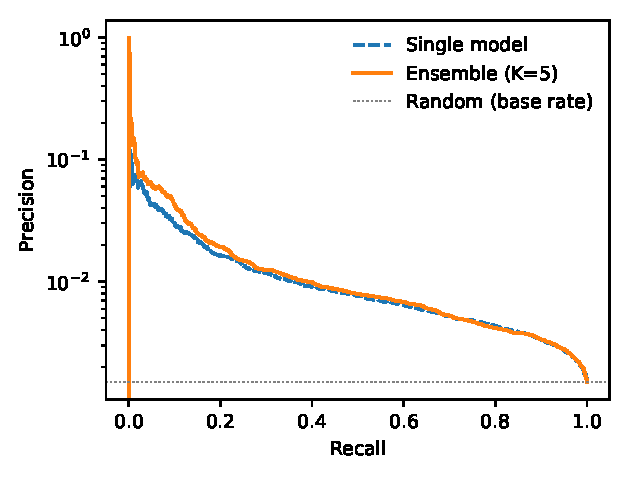
\includegraphics[width=0.48\linewidth]{figures/pr_curves.pdf}\hfill
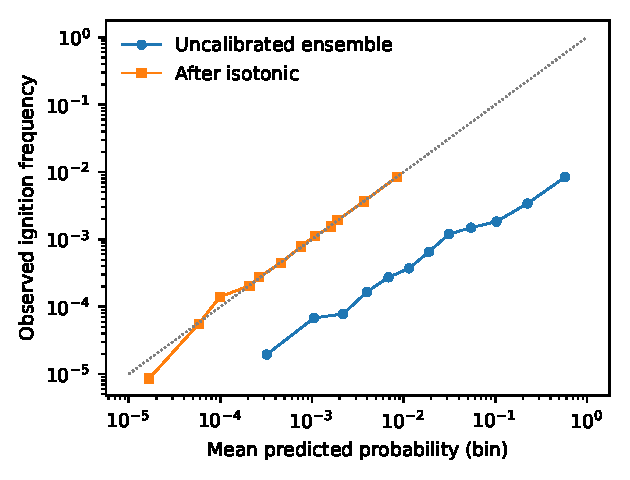
\includegraphics[width=0.48\linewidth]{figures/reliability.pdf}
\caption{Portugal temporal holdout (2024--2026). Left: precision-recall
curves (log precision axis); the ensemble dominates the single model in the
high-precision regime. Right: reliability diagram on quantile bins (log-log);
class weighting inflates raw scores by roughly an order of magnitude, and
isotonic calibration restores empirical frequencies.}
\label{fig:pr}
\end{figure}

\begin{figure}[t]
\centering
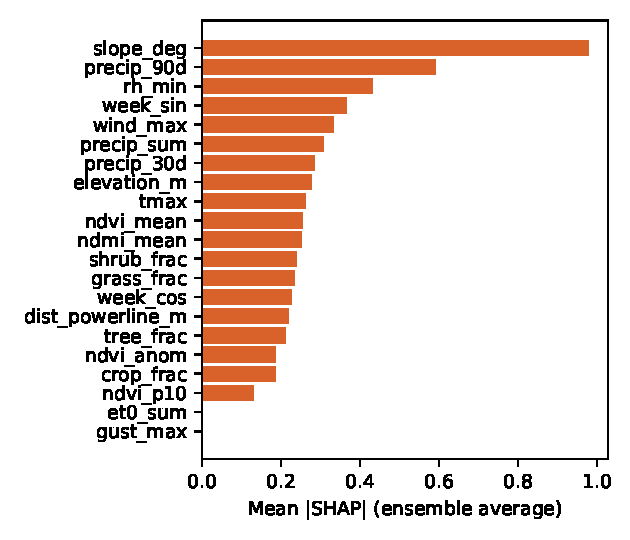
\includegraphics[width=0.48\linewidth]{figures/shap_importance.pdf}\hfill
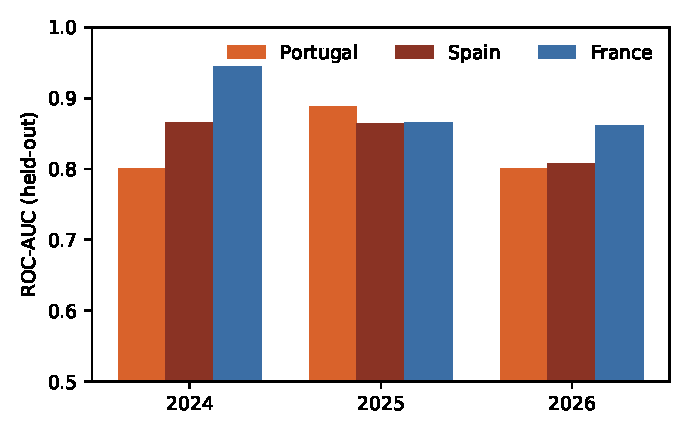
\includegraphics[width=0.48\linewidth]{figures/by_year.pdf}
\caption{Left: ensemble-averaged mean $|$SHAP$|$ feature importances on the
Portugal holdout. Right: held-out ROC-AUC by test year and region;
season-to-season variance is the dominant error source.}
\label{fig:shap}
\end{figure}

\paragraph{Calibration.} Figure~\ref{fig:pr} (right) shows the reliability
diagram. Raw class-weighted scores overstate probability by roughly an order
of magnitude; isotonic calibration aligns predicted probability with
observed frequency across four orders of magnitude. Post-calibration, the
distribution of deployed probabilities is honest but compressed (maximum
$\approx 0.05$ in a typical Portuguese week), motivating the
distribution-relative tier presentation described in
Section~\ref{sec:method}.

\paragraph{Seasonal shift dominates.} Per-year results
(Figure~\ref{fig:shap}, right) vary far more than model-choice deltas:
Portugal reaches ROC-AUC 0.889 and PR-AUC 0.0395 in the severe 2025 season
but 0.80 in the quieter 2024 and (partial) 2026 seasons, a direct
observation of the distribution-shift problem highlighted by
\citet{jiang2026eapo}. Models are most reliable exactly when fire load is
high, which is operationally fortunate, but closing the quiet-season gap,
for example through season-similarity weighted ensembling, is the clearest
future-work direction.

\section{Limitations}
\label{sec:limitations}

Weekly weather features are observed rather than forecast; a production
forecast system would substitute NWP outputs, leaving backtests unchanged.
EFFIS perimeters are MODIS-derived and under-report small fires, so labels
are a conservative subset of true ignitions, and label noise differs by
country. The evaluation is temporally but not spatially blocked; spatial
autocorrelation within a week may flatter absolute metrics, though it
affects all compared models equally. The corridor aggregation weights in
Eq.~\ref{eq:corridor} are heuristic pending corridor-level incident data,
which no public European dataset provides: corridor risk is fire risk near
the line, not a claim that the line causes ignition. Finally, isotonic
calibration is fitted on the same holdout used for reporting; because the
transform is monotone the reported ranking metrics are unaffected, but the
post-calibration reliability curve should be read as in-sample.

\section{Conclusion}

Firefinder demonstrates that operationally useful, corridor-level wildfire
risk forecasting can be built end to end from free public data and modest
models, provided the rare-event statistics are treated honestly: temporal
holdouts, base-rate-aware metrics, calibration to true likelihoods, and
uncertainty from ensemble disagreement. A seed-diverse XGBoost ensemble with
isotonic calibration currently offers the best precision-at-the-top of the
alternatives tested, and a pairwise ranking objective, despite matching the
product surface, trades away exactly the precision the product needs. The
system, data pipeline and models are open source, and the deployed
application rescores three countries daily at
\url{https://firefinder.eu}.

\bibliographystyle{unsrtnat}
\begin{thebibliography}{20}

\bibitem[Jones et al.(2022)]{jones2022global}
M.~W. Jones, J.~T. Abatzoglou, S.~Veraverbeke, et~al.
\newblock Global and regional trends and drivers of fire under climate change.
\newblock \emph{Reviews of Geophysics}, 60(3):e2020RG000726, 2022.

\bibitem[Chen and Guestrin(2016)]{chen2016xgboost}
T.~Chen and C.~Guestrin.
\newblock {XGBoost}: A scalable tree boosting system.
\newblock In \emph{Proceedings of the 22nd ACM SIGKDD International Conference
  on Knowledge Discovery and Data Mining}, pages 785--794, 2016.

\bibitem[Wang et al.(2021)]{wang2021identifying}
S.~S.-C. Wang, Y.~Qian, L.~R. Leung, and Y.~Zhang.
\newblock Identifying key drivers of wildfires in the contiguous {US} using
  machine learning and game theory interpretation.
\newblock \emph{Earth's Future}, 9(6):e2020EF001910, 2021.

\bibitem[Kondylatos et al.(2022)]{kondylatos2022wildfire}
S.~Kondylatos, I.~Prapas, M.~Ronco, et~al.
\newblock Wildfire danger prediction and understanding with deep learning.
\newblock \emph{Geophysical Research Letters}, 49(17):e2022GL099368, 2022.

\bibitem[Buch et al.(2023)]{buch2023smlfire}
J.~Buch, A.~P. Williams, C.~S. Juang, W.~D. Hansen, and P.~Gentine.
\newblock {SMLFire1.0}: a stochastic machine learning ({SML}) model for
  wildfire activity in the western {United States}.
\newblock \emph{Geoscientific Model Development}, 16(12):3407--3433, 2023.

\bibitem[Jiang and Sun(2026)]{jiang2026eapo}
E.~Jiang and W.~Sun.
\newblock Environment-adaptive preference optimization for wildfire
  prediction.
\newblock \emph{arXiv preprint arXiv:2605.12435}, 2026.

\bibitem[Lundberg and Lee(2017)]{lundberg2017shap}
S.~M. Lundberg and S.-I. Lee.
\newblock A unified approach to interpreting model predictions.
\newblock In \emph{Advances in Neural Information Processing Systems},
  volume~30, 2017.

\bibitem[Brodsky(2018)]{uber2018h3}
I.~Brodsky.
\newblock {H3}: Uber's hexagonal hierarchical spatial index.
\newblock Uber Engineering, 2018.
\newblock \url{https://h3geo.org}.

\bibitem[Sugiyama and Kawanabe(2012)]{sugiyama2012covariate}
M.~Sugiyama and M.~Kawanabe.
\newblock \emph{Machine Learning in Non-Stationary Environments: Introduction
  to Covariate Shift Adaptation}.
\newblock MIT Press, 2012.

\bibitem[Zadrozny and Elkan(2002)]{zadrozny2002transforming}
B.~Zadrozny and C.~Elkan.
\newblock Transforming classifier scores into accurate multiclass probability
  estimates.
\newblock In \emph{Proceedings of the Eighth ACM SIGKDD International
  Conference on Knowledge Discovery and Data Mining}, pages 694--699, 2002.

\bibitem[San-Miguel-Ayanz et al.(2012)]{sanmiguel2012effis}
J.~San-Miguel-Ayanz, E.~Schulte, G.~Schmuck, et~al.
\newblock Comprehensive monitoring of wildfires in {Europe}: the {European
  Forest Fire Information System (EFFIS)}.
\newblock In \emph{Approaches to Managing Disaster}. InTech, 2012.

\bibitem[Drusch et al.(2012)]{drusch2012sentinel}
M.~Drusch, U.~Del~Bello, S.~Carlier, et~al.
\newblock {Sentinel-2}: {ESA}'s optical high-resolution mission for {GMES}
  operational services.
\newblock \emph{Remote Sensing of Environment}, 120:25--36, 2012.

\bibitem[Hersbach et al.(2020)]{hersbach2020era5}
H.~Hersbach, B.~Bell, P.~Berrisford, et~al.
\newblock The {ERA5} global reanalysis.
\newblock \emph{Quarterly Journal of the Royal Meteorological Society},
  146(730):1999--2049, 2020.

\bibitem[Zanaga et al.(2022)]{zanaga2022worldcover}
D.~Zanaga, R.~Van~De~Kerchove, D.~Daems, et~al.
\newblock {ESA WorldCover} 10\,m 2021 v200, 2022.

\bibitem[Abatzoglou et al.(2025)]{abatzoglou2025climate}
J.~T. Abatzoglou, C.~A. Kolden, A.~C. Cullen, et~al.
\newblock Climate change has increased the odds of extreme regional forest
  fire years globally.
\newblock \emph{Nature Communications}, 16(1), 2025.

\end{thebibliography}

\end{document}
